% XeLaTeX

\documentclass{article}
\usepackage{ctex}
\usepackage{xypic}
\usepackage{amsfonts,amssymb}
\usepackage{multirow}
\usepackage{geometry}
\usepackage{graphicx}
\usepackage{listings}
\usepackage{lipsum}
\usepackage{courier}
\usepackage{fancyvrb}
\usepackage{etoolbox}


\linespread{1.2}
\geometry{left=3cm,right=2.5cm,top=2.5cm,bottom=2.5cm}

\makeatletter
\patchcmd{\FV@SetupFont}
  {\FV@BaseLineStretch}
  {\fontencoding{T1}\FV@BaseLineStretch}
  {}{}
\makeatother

\lstset{basicstyle=\small\fontencoding{T1}\ttfamily,breaklines=true}
\lstset{numbers=left,frame=shadowbox,tabsize=4}
%\lstset{extendedchars=false}
\begin{document}

\title{Project 4 实验报告}
\author {姓名:王凯祺 \text{ } 学号:16337233 \text{ } 班级:教务3班}
\maketitle

\section{需求分析}
实现一个选课系统(命令行程序),多用户,支持以下操作:

\subsection{管理员}

1. 添加一位教师

2. 添加一位学生

\subsection{教师}

1. 添加一门课程

2. 删除一门课程

3. 查看选中该课程的所有学生

\subsection{学生}

1. 选课

2. 退课

3. 查看选课结果

\section{实现思路}

\begin{figure}[!hbp]
	\centering
	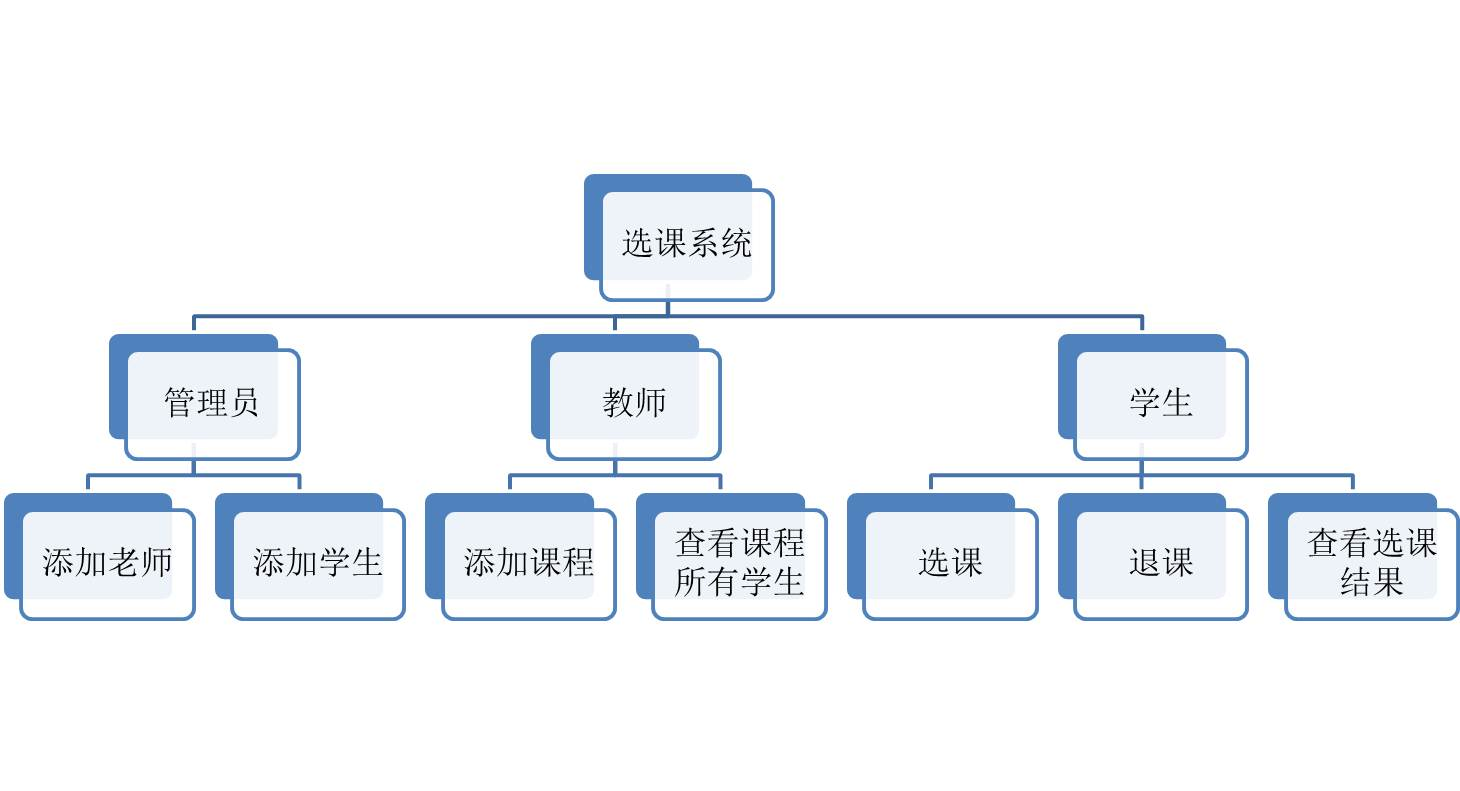
\includegraphics[scale=0.4]{S1.jpg}
\end{figure}

创建一个课程列表、人员列表的类。

添加教师、学生、课程:直接在对应类上添加即可。

查看选中该课程的所有学生:遍历一次该课程的学生名单即可。

选课和退课:在相应课程中加入该学生或者删除该学生。

查看选课结果:暴力搜索所有课程,将所有该学生的课程显示出来。

\section{较 Project 2 作出的改进}

在功能上,本次 Project 较 Project 2 \emph{几乎没有}新增或删除功能,但对整个类重新进行了定义,使得类的功能更加清晰。

\subsection{将静态变量、静态函数改为成员变量、成员函数}

Project 2 中,我对“课程列表”、“教师列表”、“学生列表”分别创建一个类。考虑到每个类仅有一个实例(更重要的是为了我写代码方便),我把里面的成员全部写成静态成员。事实上,这样写难以维护,也难以扩展,与普通的函数无异。故在本次 Project 中,我将静态成员更改为成员。

\subsection{更换容器}

Project 2 中,我选择用 vector 容器来存储课程参与人员、课程列表、人员列表。事实上,这样写效率低,而且要用更多的代码才能实现相同的功能。在本次 Project 中,我选择用 map 容器存储课程列表,用 set 容器存储课程参与人员,简化了代码更提升了效率。

\subsection{不在成员函数中与用户交互}

把与用户交互的输入输出模块从成员函数中搬到主函数中,这样可以使得整个类的功能更加清晰。

\section{对象设计}

\subsection{人员列表}

人员既可以指教师,也可以指学生。在使用时,我用此类创建了两个对象——教师和学生。

\begin{lstlisting}[language=C++]
//person.h

class person_list {
public:
    void read(string filename); // 从磁盘中的 filename 文件读取人员信息到内存
    bool add(int id, string name); // 新增一个编号为id、姓名为name的人员,并返回添加是否成功
    string id2name(int id); // 将编号转换为姓名
    void write(string filename); // 从内存写入人员信息到磁盘中 filename 文件
private:
    map <int, string> person; // first 表示编号, second 表示姓名
};
\end{lstlisting}

\subsection{课程列表}

\begin{lstlisting}[language=C++]
//course.h

struct course_b {
    int course_id;
    string name;
    int tea_id;
    string tea_name;
    set < int > stu_id; // 学生编号
    set < pair <int, string> > stu; // first 表示学生编号, second 表示学生姓名
};

class course_list {
public:
    void read(string filename); // 从磁盘中的 filename 文件读取课程列表到内存
    int add(string name, int tea_id, string tea_name); // 添加一门名称为 name 的课程,教师编号为 tea_id ,教师姓名为 tea_name ,并返回课程 ID
    int del(int course_id); // 删除课程 ID 为 course_id 的课程,并返回删除是否成功
    bool is_select(int course_id, int stu_id); // 返回学生编号为 stu_id 的学生是否选择了课程编号为 course_id 的课程
    bool select(int course_id, int stu_id, string stu_name); // 学生编号为 stu_id 、学生姓名为 stu_name 的学生选择课程编号为 course_id 的课程,并返回选课是否成功
    bool unselect(int course_id, int stu_id, string stu_name); // 学生编号为 stu_id 、学生姓名为 stu_name 的学生退出课程编号为 course_id 的课程,并返回退课是否成功
    void write(string filename); // 从内存写入课程列表到磁盘中 filename 文件
    string get_all_course(int tea_id = -1, int stu_id = -1); // 获取关于该用户的所有课程
    string get_course_info(int course_id); // 获取某门课的信息
private:
    map< int, course_b > c; // first 表示课程编号, second 表示课程的详细信息
};
\end{lstlisting}

\section{输入与输出}

使用标准输入输出与用户交互。

使用文件输入输出与硬盘数据交互:初始化时从硬盘读取数据,每完成一个操作,立即将修改写入文件。

\end{document}
















